\documentclass[12p]{amsart}
\usepackage[margin=1in]{geometry}
\renewcommand{\baselinestretch}{1}

\usepackage[utf8]{inputenc}
\usepackage[mathscr]{eucal}
\usepackage{enumerate}
\usepackage{amssymb}
\usepackage{amsmath}
\usepackage{amsthm}
\usepackage{bm}
\usepackage{url}
\usepackage{arydshln}
\usepackage{mathtools}

\usepackage{pgf,tikz}
\usetikzlibrary{arrows,matrix}
\usetikzlibrary{arrows.meta,math}

\numberwithin{equation}{section}
\theoremstyle{plain}
\newtheorem{thm}{Theorem}[section]
\newtheorem{lemma}[thm]{Lemma}
\newtheorem{prop}[thm]{Proposition}
\newtheorem{cor}[thm]{Corollary}
\newtheorem{claim}[thm]{Claim} 
\newtheorem{fact}[thm]{Fact}
\newtheorem{question}[thm]{Question}

\theoremstyle{definition}
\newtheorem{defn}[thm]{Definition}
\newtheorem{ex}[thm]{Example}
\newtheorem{notation}[thm]{Notation}
\newtheorem{conject}[thm]{Conjecture}
\newtheorem{remark}[thm]{Remark}
\newtheorem{example}[thm]{Example}

\newcommand{\Or}{\mathcal{O}}
\newcommand{\Z}{\mathbb {Z}}

\newcommand{\mbf}{\mathbf}

\DeclareMathOperator{\im}{im}
\DeclareMathOperator{\coker}{coker}

% Feel free to make a version of this command for other notes
%%%%%%%%%%%%%%%%%%%%%%%%%%%%%%%%%%%
\newcommand{\TODO}[1]{\textcolor{red}{TODO: #1}}

\newcommand{\anote}[1]{\par 
  \framebox{\begin{minipage}[c]{0.95 \textwidth}\color{blue} ALEX'S NOTE:
      #1 \color{black}\end{minipage}}\par}

\newcommand{\mnote}[1]{\par 
  \framebox{\begin{minipage}[c]{0.95 \textwidth}\color{orange} MIKE'S NOTE:
      #1 \color{black}\end{minipage}}\par}

\newcommand{\dnote}[1]{\par 
  \framebox{\begin{minipage}[c]{0.95 \textwidth}\color{magenta} DAVE'S NOTE:
      #1 \color{black}\end{minipage}}\par}
%%%%%%%%%%%%%%%%%%%%%%%%%%%%%%%%%%%%


\title{Circuit-Cocircuit Reversal Rank on Regular Matroids}
\author{}
\date{}

\begin{document}

\begin{abstract}TODO \end{abstract}

\maketitle
\anote{Here's a note from me.}
\mnote{Here's a note from Mike! Feel free to change the color.} 
\dnote{Here's a note from Dave! Feel free to change the color.} 
\section{Introduction}
Here is some code that Mike wrote up. 
\url{https://mikeion.github.io/graph-problems/}. I also included a pdf of Dave's writeup as a file in this project. 

At a high level, the motivation for this project is the same as my motivation for the $R_{10}$ matroid project.

\begin{question}
    What are some properties of \emph{graphic/co-graphic matroids} that \textbf{do not} generalize naturally to the setting of \emph{regular matroids} (especially properties relating to \emph{sandpile groups}). 
\end{question}

Beyond considering graphs and regular matroids, we can also distinguish between planar and non-planar graphs. 

Every graph $G$ has a corresponding \emph{graphic matroid}. This matroid is also \emph{cographic} if and only if $G$ is planar. All graphic or cographic matroids are \emph{regular}, but there are also regular matroids that are neither graphic nor cographic (such as the matroid $R_{10}$). See Figure~\ref{fig:Venn} for a depiction of these different kinds of matroids. 

\begin{figure}
\begin{center}
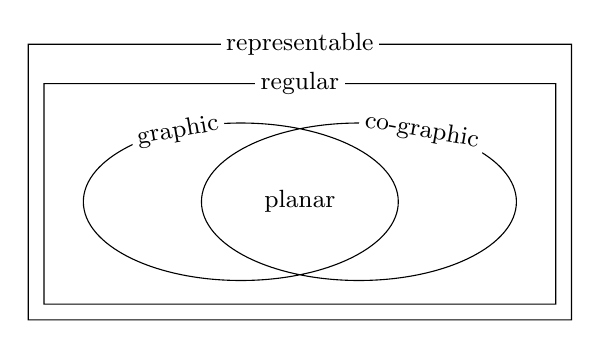
\begin{tikzpicture}

\draw (0,0) ellipse (2cm and 1cm)
      (1.5,0) ellipse (2cm and 1cm)
      (-2.5,-1.3) rectangle (4,1.5)
      (-2.7,-1.5) rectangle (4.2,2);
      \node[draw = none, fill =white,inner sep = 2pt,rotate = 10]  at (-.8,.9) {\small{graphic} };
      \node[draw = none, fill =white,inner sep = 2pt,rotate = -10]  at (2.3,.9) {\small{co-graphic} };
      \node[draw = none, fill =none]  at (.75,0) {\small{planar} };
      \node[draw = none, fill =white,inner sep = 2pt]  at (.75,1.5) {\small{regular} };
      \node[draw = none, fill =white,inner sep = 2pt]  at (.75,2) {\small{representable} };
\end{tikzpicture}
\caption{This is a Venn diagram of the classes of matroids that are relevant for this article.}\label{fig:Venn}
\end{center}
\end{figure}

\section{Circuit Reversals on Graphs} 
\anote{Most people use \emph{cycle}/\emph{cocycle} in place of \emph{circuit}/\emph{cocircuit} when restricting to graphs, but I just say circuit/cocircuit everywhere. I also don't always use the hyphen.} 
Given a graph $G$, let $\mathcal{C}(G)$ be the set of circuits of $G$. Let $\mathcal O$ and $\mathcal O'$ be orientations on the edges of $G$, and let $\mathbf C\subseteq \mathcal C(G)$ be a collection of circuits. We say that a circuit $C$ is \emph{compatible} with $\mathcal O$ if the edges of $C$ form a \emph{signed circuit} of $\mathcal O$. We write $\mathcal O \xleftrightarrow{~~\mathbf C~~} \mathcal O'$ if one can reach $\mathcal O$ from $\mathcal O'$ by reversing circuits from $\mathbf C$ that at each step are compatible with the current orientation. An orientation $\mathcal O$ is called \emph{totally cyclic} if every edge is part of a circuit. 


The following definition is new for this paper. \anote{lots of names and notation could use some improvement, but I want to get some ideas down.} 
\begin{defn}
    For a graph $G$, the \emph{circuit reversal rank} is the minimum possible size of a collection $\mathbf C\subseteq \mathcal C(G)$ such that for every pair of totally cyclic orientations $\mathcal O,\mathcal O'$, the following condition is satisfied:
    \begin{equation}\label{eq:generators} \mathcal O \xleftrightarrow{~~\mathbf C~~} \mathcal O'\iff \mathcal O \xleftrightarrow{\mathcal{C}(G)} \mathcal O'.\end{equation}
\end{defn}
    


Given an orientation $\mathcal O$ and a compatible circuit $C$, write ${}_{C} \mathcal O$ for the orientation obtained by reversing the circuit $C$. 
\begin{lemma}
    A set $\mathbf C\subseteq \mathcal C(G)$ satisfies~\eqref{eq:generators} if and only if for every totally cyclic orientation $\mathcal O$ and every circuit $C$ that is compatible with $\mathcal O$, we have $\mathcal O \xleftrightarrow{~~\mathbf C~~} {}_{C} \mathcal O$ 
\end{lemma}


\begin{prop}
    Suppose that $G$ has $n$ vertices and $m$ edges. The reversal-generating rank of $G$ is at least $m-n+1$. 
\end{prop}

This value $m-n+1$ is sometimes called the \emph{genus} of $G$ (although this term is also sometimes used for the minimal genus surface that $G$ embeds into). This is also the rank of the circuit lattice. 

\begin{prop}
    When $G$ is a planar graph, the circuit reversal rank is exactly $m-n+1$. 
\end{prop}
\begin{proof}[sketch] Consider an embedding of $G$ in the plane. We can have the generators be the ``faces''. To reverse a circuit, we can reverse all of the circuits inside of it. 
\end{proof}

The goal will be to show that this is not always true for non-planar graphs (which correspond to matroids that are not cographic). However, there is a set of graphs where this minimum is hit. 

\begin{prop}
    For any $n$, the reversal-generating rank of $K_n$ is exactly $m-n+1$, which is also equal to $(n-2)(n-1)/2$. 
\end{prop}
\begin{proof}[sketch] We can let $\mathbf C$ be the set of all triangles containing a given vertex. I have a nifty argument for why this will always work, but I think it would be easier to explain verbally. 
\end{proof}

\begin{prop}
    The reversal-generating rank of $K_{3,3}$ is 5, even though $m-n+1 = 4$.
\end{prop}
\begin{proof}
Label the bipartition of $K_{3,3}$ as $L = \{L_0, L_1, L_2\}$ and $R = \{R_0, R_1, R_2\}$.
Since $K_{3,3}$ has 9 edges and each vertex has degree 3, every totally cyclic orientation has each vertex with out-degree 1 or 2.
Let $\mathcal{C}^*$ denote the reversal class of all TCOs with $\deg^+(L_i) = 2$ for every $i$ (so $\deg^+(R_j) = 1$ for every $j$).
Direct enumeration gives $|\mathcal{C}^*| = 6$.

\begin{claim}\label{claim:K6}
The subgraph of the flip graph induced on $\mathcal{C}^*$ is the complete graph $K_6$, and the 15 edges carry 15 mutually distinct circuit labels --- precisely the full set of circuits of $K_{3,3}$ (nine 4-cycles and six 6-cycles).
\end{claim}

\begin{proof}[Proof of Claim]
For each of the $\binom{6}{2} = 15$ pairs $(\mathcal{O}, \mathcal{O}') \subset \mathcal{C}^*$ one checks that the symmetric difference $\mathcal{O} \triangle \mathcal{O}'$ is a directed circuit in $\mathcal{O}$, so every pair is connected by a single circuit reversal.
One further checks that the 15 resulting circuit masks are all distinct and account for all 15 circuit masks that appear across any TCO of $K_{3,3}$. (Verified by exhaustive enumeration; see the accompanying code.)
\end{proof}

\noindent\textbf{Lower bound.} Let $\mathbf{C}$ be any generating set. The $\mathbf{C}$-restricted flip graph must span $\mathcal{C}^*$, so the edges of the $K_6$ on $\mathcal{C}^*$ whose labels lie in $\mathbf{C}$ must form a connected spanning subgraph. By Claim~\ref{claim:K6} the labels of these 15 edges are all distinct and cover every circuit of $K_{3,3}$, so $\mathbf{C}$ contributes at most one edge per mask and thus exactly $|\mathbf{C}|$ edges. A spanning connected subgraph of $K_6$ requires at least $5$ edges (a spanning tree), so $|\mathbf{C}| \geq 5$.

\noindent\textbf{Upper bound.} Label the nine 4-cycles by the pair of left vertices and pair of right vertices they pass through:
\[
\begin{array}{c|ccc}
& R_0 R_1 & R_0 R_2 & R_1 R_2 \\ \hline
L_0 L_1 & a & b & c \\
L_0 L_2 & d & e & f \\
L_1 L_2 & g & h & i
\end{array}
\]
The set $\mathbf{C} = \{a, b, d, e, i\}$ is a generating set of size 5 (verified computationally). There are exactly 9 such minimal sets, all consisting of five 4-cycles and no 6-cycle.
\end{proof}
\mnote{The lower bound uses the $K_6$ structure of the class $\mathcal{C}^*$: because all 15 circuit masks of $K_{3,3}$ appear as distinct edge-labels on this $K_6$, any generating set must supply at least a spanning tree worth of edges, giving $|\mathbf{C}| \geq 5$. The claim is verified by the script \texttt{k33\_key\_argument.py}.}


\section{Additional directions} 

It would be nice to get a characterization of which graphs have a circuit reversal rank of $m-n+1$ (and what the rank is in general). I would also like to move from graphs to regular matroids. In this context, we can consider cocircuit reversals on acyclic orientations as well (for graphs, it always achieves the minimum of $n-1$). Furthermore, we could consider orientations that aren't totally cyclic or acyclic. For an arbitrary orientation, the graph/matroid splits into a totally cyclic portion and an acyclic portion (where each can be made up of disjoint pieces). It could be interesting to look at all of the possible ways to partition a graph/matroid into acyclic/totally cyclic portions (or this could be trivial/ already studied). 

\section{Background} 
\anote{All of this is old material from a draft of my paper with Mike, but it might give some useful background.}
\subsection{Regular Matroids}
For this article, we do not need the full generality of matroid theory. Instead, we can restrict to \emph{representable matroids}, which can be described in terms of a matrix. 

Let $\mathcal A$ be a matrix, $n$ be the number of columns of $\mathcal A$, and $F$ be a field. The \emph{ground set} $E$ is a set whose elements correspond to the columns of $\mathcal A$. If a subset of $E$ corresponds to columns which are linearly independent over $F$, then it is called an \emph{independent} set. The maximal independent sets are called \emph{bases}, and the collection of bases is called $\mathbf B$.
\begin{defn}The \emph{matroid represented by $\mathcal A$ over $F$} is the pair $(E,\mathbf B)$, where $E$ and $\mathbf B$ are defined above.
\end{defn}

\begin{ex}\label{ex:kylematroid}
    Consider the matrix \[\mathcal A = \begin{bmatrix} 1 & 0 & 0 & 1 & 1\\
    0 & 1 & 0 & -1 & 0 \\
    0 & 0 & 1 & 0 & -1 \end{bmatrix}.\]
    We will calculate the matroid represented by $\mathcal A$ over $\mathbb R$. Let $E = \{1,2,3,4,5\}$ be the ground set. Since the matrix has 3 rows, a collection of more than 3 columns cannot be linearly independent. Furthermore, of the 10 subsets of size 3, the only linearly dependent subsets are $\{1,2,4\}$ and $\{1,3,5\}$. In particular, the bases of this matroid are given by $\mathbf B = \{\{1,2,3\},\{1,2,4\},\{1,2,5\},\{1,3,5\},\{1,4,5\},\{2,3,4\},\{2,4,5\},\{3,4,5\}\}$. 
\end{ex}

A matroid is \emph{representable} if it can be represented by some matrix over some field. The classical definition of a \emph{regular matroid} is a matroid that is representable over \emph{any} field. However, we will use the following definition, which was proven equivalent by Tutte~\cite{Tutte}. 
\begin{defn}
    A \emph{regular matroid} is a matroid that is representable over $\mathbb R$ by a \emph{totally unimodular} matrix $\mathcal A$. A \emph{totally unimodular} matrix is an integer matrix such that every minor is in the set $\{0, 1,-1\}$. 
\end{defn}

For example, it is straightforward to check that the matrix from Example~\ref{ex:kylematroid} is totally unimodular, so the corresponding matroid is regular. 

One way to obtain a totally unimodular matrix is from a graph. Begin with any connected graph $G$ and choose an ordering for the vertices and edges, as well as an orientation for each edge. Then, let $A(G)$ be the \emph{signed adjacency matrix} of $G$ defined by
\[A(G)_{ij} = \begin{cases} 1 & \text{if edge $j$ is incident to vertex $v_i$, and is directed \textit{away from} $v_i$.}\\
-1 & \text{if edge $j$ is incident to vertex $v_i$, and is directed \textit{towards} $v_i$.}\\
0 & \text{otherwise.}\end{cases}\]

\begin{defn}
    Given a graph $G$, the \emph{matroid associated with $G$} is the matroid represented by $A(G)$ over $\mathbb R$. A matroid that can be obtained from a graph in this way is called a \emph{graphic matroid}.
\end{defn}

Note that the ordering of the vertices and the orientation of the edges has no impact on the resulting matroid, and permuting the edges just permutes the ground set in the same way. See Figure~\ref{fig:graphic_matroid} for an example of a graph and the corresponding signed adjacency matrix. 

\begin{figure}
\begin{center}
	$G = 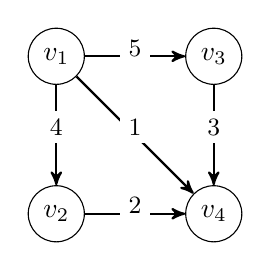
\begin{tikzpicture}[anchor = base, baseline]
			\tikzstyle{o}=[circle,draw]
				\node [o] (1) at (0,1) {$v_1$};
				\node [o] (2) at (0,-1) {$v_2$};
				\node [o] (3) at (2,1) {$v_3$};
                \node [o] (4) at (2,-1) {$v_4$};
				\draw [thick,->,>=stealth',] (1) to node[fill = white,inner sep=3pt]{\small $1$} (4);
                \draw [thick,->,>=stealth',] (2) to node[fill = white,inner sep=3pt]{\small $2$} (4);
                \draw [thick,->,>=stealth',] (3) to node[fill = white,inner sep=3pt]{\small $3$} (4);
                \draw [thick,->,>=stealth',] (1) to node[fill = white,inner sep=3pt]{\small $4$} (2);
                \draw [thick,->,>=stealth',] (1) to node[fill = white,inner sep=3pt]{\small $5$} (3);
	\end{tikzpicture}
    \hspace{ 2 cm}
A(G) = \begin{bmatrix}1 & 0 & 0 & 1 & 1\\
    0 & 1 & 0 & -1 & 0 \\
    0 & 0 & 1 & 0 & -1 \\
    -1 & -1 & -1 & 0 & 0\end{bmatrix}$
    \caption{On the left is a graph $G$ where the edges are oriented, and the vertices and edges are each ordered. On the right is the singed incidence matrix of the graph, which we denote $A(G)$. The rows correspond to vertices and the edges correspond to edges, each in numerical order. The matroid represented by $A(G)$ is called the \emph{graphic matroid associated with $G$}.} 
    \label{fig:graphic_matroid}
    \end{center}
\end{figure}

It is well known that the signed adjacency matrix of any graph must be totally unimodular. As a consequence, this means that every graphic matroid is a regular matroid. Furthermore, the \emph{bases} of the matroid represented by $A(G)$ correspond precisely to the \emph{spanning trees} of $G$ (i.e., the maximal collections of edges with no cycles). 

Another property of signed adjacency matrices of graphs is that the row rank is always one less than the number of rows. This corresponds to the fact that it only takes $k-1$ edges to connect $k$ vertices. A consequence of this fact is that any single row of $A(G)$ can be removed without impacting the matroid represented by $A(G)$. 

\begin{ex}\label{ex:remove_row}
    Notice that the matrix $\mathcal A$ from Example~\ref{ex:kylematroid} is equivalent to $A(G)$ from Figure~\ref{fig:graphic_matroid}, except with the bottom row removed. By the discussion in the previous paragraph, this means that the matroid represented by $\mathcal A$ over $\mathbb R$ is the graphic matroid associated with $G$. 

    Furthermore, the bases of this matroid correspond precisely to the spanning trees of $G$. Indeed, the 8 spanning trees of $G$ correspond precisely to the triples of edges other than $\{1,2,4\}$ or $\{1,3,5\}$.
\end{ex}

Given a matroid $\mathcal M = (E,\mathbf B)$, we can obtain a new matroid $\mathcal M^*=(E,\mathbf B^*)$ by using the same ground set, and letting $B^* \in \mathbf B^*$ if and only if $E \setminus B^* \in \mathbf B$. 

\begin{defn}
    A \emph{co-graphic matroid} is a matroid that is dual to a graphic matroid. A \emph{planar matroid} is a matroid that is both graphic and cographic. 
\end{defn}

Note that planar matroids are precisely the graphic matroids associated with \emph{planar graphs}. See Figure~\ref{fig:Venn} for a Venn diagram of all of the classes of matroids that are relevant in this paper. 





\subsection{Orientations, Cycles, and Cocycles} 

An \emph{Orientation} $\mathcal O(G)$ on a graph $G$ is a choice of direction of each edge of $G$. A \emph{signed cycle} is a path of directed edges that returns to where it started (and does not cross itself before). A \emph{signed cocycle} is a minimal cut where all edges are directed consistently. 

\anote{This is a special case of Farkas' lemma. We can decide how we want to cite it.}
\begin{prop}\label{prop:cycle-cocycle} 
    Let $G$ be a graph, $\mathcal O(G)$ be an orientation, and $e$ be an edge of $G$. Then, there must either be a signed cycle containing $e$ or a signed cocycle containing $e$ but not both. 
\end{prop}

Given an orientation $\mathcal O(G)$, let 
\[\mathcal O(G)_{cyc} = \{e \in E(G) \ \mid \ \text{e is in a signed cycle}\}\text{, and}\]
\[\mathcal O(G)_{cocyc} = \{e \in E(G) \ \mid \ \text{e is in a signed cocycle}\}\]

\begin{defn}
    If $\mathcal O(G)_{cyc} = E(G)$, then we say that $\mathcal O(G)$ is \emph{totally cyclic}. If $\mathcal O(G)_{cocyc} = E(G)$, then we say that $\mathcal O(G)$ is \emph{acyclic}.
\end{defn}

These same definitions also work for regular matroids. In this context, we use the words \emph{circuit} and \emph{cocircuit} in place of \emph{cycle} and \emph{cocyle} respectively. Given a totally unimodular matrix $\mathcal A$ that represents a regular matroid, an orientation can be thought of as a choice of sign for each column of $\mathcal A$. If a collection of columns can be added with the signs specified from the orientation, then we say that they form a \emph{signed circuit}. \emph{Signed Cocircuits} are a little bit harder to describe, but they are dual objects. 


\bibliographystyle{alpha}
\bibliography{biblio}
\end{document}